\documentclass[a4paper,10pt,twocolumn]{article}
\usepackage[utf8]{inputenc}
\usepackage[UKenglish]{babel}	% english word division
\usepackage[automark]{scrpage2}
\usepackage{amsmath}
\usepackage{listings}			% source code support
%\usepackage{fixltx2e}			% textsubscript command for older latex distributions
\usepackage{color} 				% Colour support
\usepackage[dvipsnames]{xcolor}	% More predifined colours
\usepackage{cite}				% Citation
% figure support
\usepackage{graphicx}
\graphicspath{ {./} }
\usepackage{geometry}
\geometry{top=25mm, left=25mm, right=25mm, bottom=25mm, headsep=10mm,footskip=12mm}
%\usepackage{float}
\pagestyle{scrheadings}
\usepackage{multirow}
\ihead{Implementation of PrefixSpan in Apache Flink} %top left
\ohead{J. Röwekamp, T. Du} %top right
\cfoot{\pagemark}
\setheadsepline[500pt]{.6pt}
\setlength{\skip\footins}{3mm}
\raggedbottom

% add space after paragraph
\setlength{\parskip}{0.5em}

\usepackage[pdftitle={Implementation of PrefixSpan in Apache Flink},pdfsubject={Frequent Pattern Mining - PrefixSpan approach},pdfauthor={Jens Roewekamp, Tianlong Du},pdfkeywords={PrefixSpan, Apache Flink, Apache Spark, TU-Berlin, EIT Digital Master School},bookmarks=true,hyperindex=false,colorlinks=true,linkcolor=black,urlcolor=black,citecolor=black,bookmarksopen=flase,linktoc=none]{hyperref}
\hypersetup{pdfpagemode=UseNone}

\author{\href{mailto:j.roewekamp@campus.tu-berlin.de}{Jens Röwekamp}, \href{mailto:du_tianlong@hotmail.com}{Tianlong Du}}
\title{Implementation of PrefixSpan in Apache Flink}
% \date{} % do not show date
\setlength{\parindent}{0pt}
% (3-8 pages in double column)

\lstset{
	% numbers=left,
	% numberstyle=\tiny,
	stepnumber=1,
	% numbersep=5pt,
	language=Java,
	backgroundcolor=\color{white},
	commentstyle=\color{LimeGreen},
    keywordstyle=\color{magenta},
    numberstyle=\tiny\color{Gray},
    stringstyle=\ttfamily\color{Orchid},
	basicstyle=\ttfamily\scriptsize,
	showstringspaces=false,
	breaklines=true,
	% captionpos=b
}

\begin{document}
% generates the title
\maketitle
% start first section

\section*{Abstract}
Data mining is commonly used by retail organizations to solve decision support problems and mining frequent items is usually among the first steps. In this paper, we show the implementation of a sequential pattern mining algorithm called PrefixSpan in Apache Flink and the experimental evaluation comparing with Apache Spark. The Flink implementation converts the recursive algorithmn to an iteration operation to execute parallel. The disk space needed for candidate patterns is the bottleneck of the approach and needs to be improved in the future.

\section{Introduction}
% <a(abc)(ac)d(cf)>
% <(ad)c(bc)(ae)>
% <(ef)(ab)(df)cb>
% <eg(af)cbc>

% Gives the backgroud meaning.
% Definations.
% Problem statement.

Retail organizations usually collect and store massive amounts of sales data. In one transaction date, customer-id and the items bought are recorded. Data mining can be used on massive data to solve decision support problems. If a customer bought something whilst online shopping, for example a SanDisk USB3.0 64GB pen drive, retailers would give a recommend, like ``customers who bought this item also bought: \dots" To give this recommend, the recommended items must be frequently bought together with the ones which the customer bought. This can be queried from the ``frequently bought together items" database. To generate this database, we need to find out frequent patterns from the transaction database. Mining frequent items is usually among the first steps to analyze a large-scale dataset. \\
In this project, we implemented a sequential pattern mining algorithm called PrefixSpan \cite{PrefixSpan} in Apache Flink \cite{Flink} and compared its performance with a reference implementation in Apache Spark \cite{Spark}, which is another platform for the distributed processing of massive amounts of data.

Here we use the same definition as in the original paper. \cite{PrefixSpan}

% add more definitions needed here
Let $I=\{i_1, i_2,\ \ldots \ ,i_n\}$ be a \emph{set} of all \textbf{items}.

An \textbf{itemset} is a \emph{subset} of items. % add more emph like this one.

A \textbf{sequence} is an \emph{ordered} list of itemsets. A sequence s is denoted by $\langle s_1 s_2 \cdots s_l\rangle$, where s\textsubscript{j} is an itemset. s\textsubscript{j} is also called an element of the sequence, and denoted as ($x_1 x_2 \cdots x_m)$, where x\textsubscript{k} is an item. For brevity, the brackets are omitted if an element has only one item, i.e. element (x) is written as x.

The number of instances of items in a sequence is called the \textbf{length} of the sequence. 
%A sequence with length l is called an l-sequence.

A \textbf{sequence database} \textit{S} is a set of tuples $\langle$sid, s$\rangle$, where sid is a sequence\_id and s a sequence.

The \textbf{support} of a sequence $\alpha$  in a sequence database \textit{S} is the number of tuples in the database containing  $\alpha$.

Given a positive integer \textit{min\_support} as the support threshold, a sequence $\alpha$ is called a \textbf{sequential pattern} in sequence database \textit{S} if $support_S (\alpha) \geq  min\_support$.

Given a sequence $\alpha=\langle e_1 e_2 \cdots e_n \rangle$, a sequence $\beta=\langle e'_1 e'_2 \cdots e'_m\rangle \left(m\leq n\right)$ is called a \textbf{prefix} of $\alpha$ if and only if
\begin{enumerate}
\item $e'_i = e_i$  for $\left( i \leq m -1 \right)$ and
\item $e'_m \subseteq e_m$ and
\item all the frequent items in ($e_m - e'_m $) are alphabetically after those in $e'_m$.
\end{enumerate}
For example, $\langle a \rangle, \langle aa \rangle, \langle a(ab) \rangle \ and \  \langle a(abc)\rangle$ are prefixes of sequence \textit{s} $ =\langle a(abc)(ac)d(cf)\rangle $, but neither $\langle ab \rangle$  nor $\langle a(bc) \rangle$ is considered as a prefix if every item in the prefix $\langle a(abc)\rangle$  of sequence \textit{s} is frequent in \textit{S}.

Let $\beta$ be be the prefix of $\alpha$, the following part in the sequence after the prefix as sequence $\gamma$ is called \textbf{suffix} with regards to prefix $\beta$. The relation of sequence $\alpha$, prefix $\beta$ and suffix $\gamma$ is denoted as $\alpha = \beta \cdot \gamma $.

Let $\alpha$ be a sequential pattern in a sequence database \textit{S}. The $\alpha$-\textbf{projected database}, denoted as $S|_\alpha$ , is the collection of suffixes of sequences in \textit{S} with regards to prefix $\alpha$.

\textbf{Problem statement:} Given a sequence database and the min\_support threshold, sequential pattern mining is to find the complete set of sequential patterns in the database.

% Algorithm history can be introduced here.

% Organization of the paper: 
Our paper proceeds as follows: Firstly, the algorithm detail is represented. Then the implementation in Apache Flink is shown. Afterwards a case study is introduced to compare the performance with a reference implementation in Apache Spark. At last, the paper ends with a conclusion.

\section{Algorithm detail} \label{algorithmDetail}
% fixed order
Given a sequence database, the first step is to fix the order in itemsets. Because items in an itemset can be listed in any order, one can fix the order of items within each itemset to avoid checking every possible combination of a potential candidate sequence. With such a convention the expression of a sequence is unique. For example, instead of $\left<a(bac)(ca)d(fc)\right>$, the items can be listed alphabetically in itemsets as $\left<a(abc)(ac)d(cf)\right>$.

% first scan
% FreeSpan is based on the following property:
% If an itemset X is infrequent, any sequence whose projected itemset is a superset of X cannot be a sequential pattern.
Secondly, we start a first scan to find the length-1 frequent items. Infrequent items are filtered out because of the following property: A sequence whose prefix is an infrequent sequence can't be a frequent sequential pattern.

% need more detail here
Next, we use database projection to do divide and conquer. According to the set of frequent items, the complete set of sequential patterns can be divided into disjoint subsets. For each basic frequent item used as a prefix, we make a projected sequence database and scan the projected database to find its length-1 frequent patterns. The new pattern either can be assembled to the last element of the prefix to form a length-2 sequential pattern $\langle$ (ab) $\rangle$, or can be appended to the prefix to form a length-2 sequential pattern $\langle$ ab $\rangle$. Recursively, the projected database can be further projected by the respective new patterns to find length-3, length-4, length-5, \dots, patterns. So the length of frequent pattern grows by 1 after each scan. The mining process ends until no more frequent patterns are found.

The following pseudo-code shows the recursive mining process:

% put the code at top of the page to have page-wide or in column if possible
% the font is not right
\begin{lstlisting}[language=Java] 
// pseudocode
PrefixSpan(prefix,sequence_db){
  // find new freqeunt pattern
  length_one_patterns=FindLengthOnePattern(sequence_db)
  // devide and conquer
  for(pattern in length_one_patterns){
    frequent_pattern=combine(prefix,pattern)
    // collect result 
    output frequent_pattern
    // project new sequence database
    projected_db=sequence_db.project(pattern)
    PrefixSpan(frequent_pattern,projected_db)
  }
}
// to call it
PrefixSpan("", sequence_db)
\end{lstlisting}

% Pseudoprojection
The major cost of PrefixSpan is database projection. Pseudoprojection is used to improve performance. Instead of performing physical projection, one can register the index (or identifier) of the corresponding sequence and the starting position of the projected suffix in the sequence. However, because random access disk space is costly, if the original sequence database or the projected databases is too large to fit into main memory (disk-based accessing situation), physical projection should be applied. Whenever the projected databases can fit in main memory, then use pseudoprojection.

% Input: A sequence database S, and the minimum support threshold min\_support.
% Output: The complete set of sequential patterns

\section{Flink Implementation}
As Flink in its current version 0.10.1 doesn't offer native mechanisms to execute recursive functions, we used two different approaches to implement the PrefixSpan algorithm. The first uses Java recursion, which calls the regarding Flink functions. The second transforms PrefixSpan's recursive divide and conquer approach to an iterative one and uses Flink's Delta Iteration to be executed natively.

\subsubsection*{Input Format}
To implement the PrefixSpan algorithm we defined our sequence database format of a DataSet$\left\langle Tuple2\left\langle Long,int[\ ]\right\rangle\right\rangle $ where the first entry is the sequence id and the second the regarding sequence. Zeros were used as itemset delimiter and needed to begin and end a sequence. To be able to use different input sources we defined an InputDecoder interface which is responsible for parsing the input source into our sequence database format. Furthermore we implemented four different Decoder classes which implement the InputDecoder interface and are used for both, the recursive and iterative, approaches.\\
The \textit{DummyInputDecoder} defines three sample databases to test if the PrefixSpan algorithm is implemented correctly.\\
The \textit{PlainInputDecoder} transforms comma separated input files of the format ``sequence\_id, 0, first item, second item, 0, third item, \dots, nth item, 0" into the database format.\\
The \textit{BigBenchInputDecoder} transforms BigBench's \cite{BigBench} store\_sales.dat, which stores customer purchases, into the database format.\\
The \textit{IBM\_DataGeneratorInputDecoder} transforms customer purchase files generated by IBM's quest data generator \cite{IBMDataGenerator} into the database format.

\subsection{Recursive approach}
The recursive implementation of the PrefixSpan algorithm was mostly analogue to the pseudocode stated in section \ref{algorithmDetail}.\\
First all frequent length-1 items are detected by flatMapping the database, grouping by the prefix, summing up the support of each prefix and filtering the infrequent prefixes.\\
Afterwards all infrequent items were deleted from the database to reduce the further amount of projections.\\
In a third step the recursion was started to find all frequent sub-patterns for each frequent length-1 item. Here MapReduce techniques and sequence position pointers were used to calculate the support of each item.\\
In the end the results were collected, sorted and written to a csv file for further access.

The source code of this implementation can be found in our Github repository. \cite{GithubRecursive}

\subsection{Iterative approach}
Flink programs implement iterative algorithms by defining a step function and embedding it into an iteration operator to execute iterations in a massively parallel fashion. Here we use the \textbf{Delta Iterate} operator to implement the PrefixSpan algorithm. The Delta Iterate model is explained below.

\begin{figure}[h]
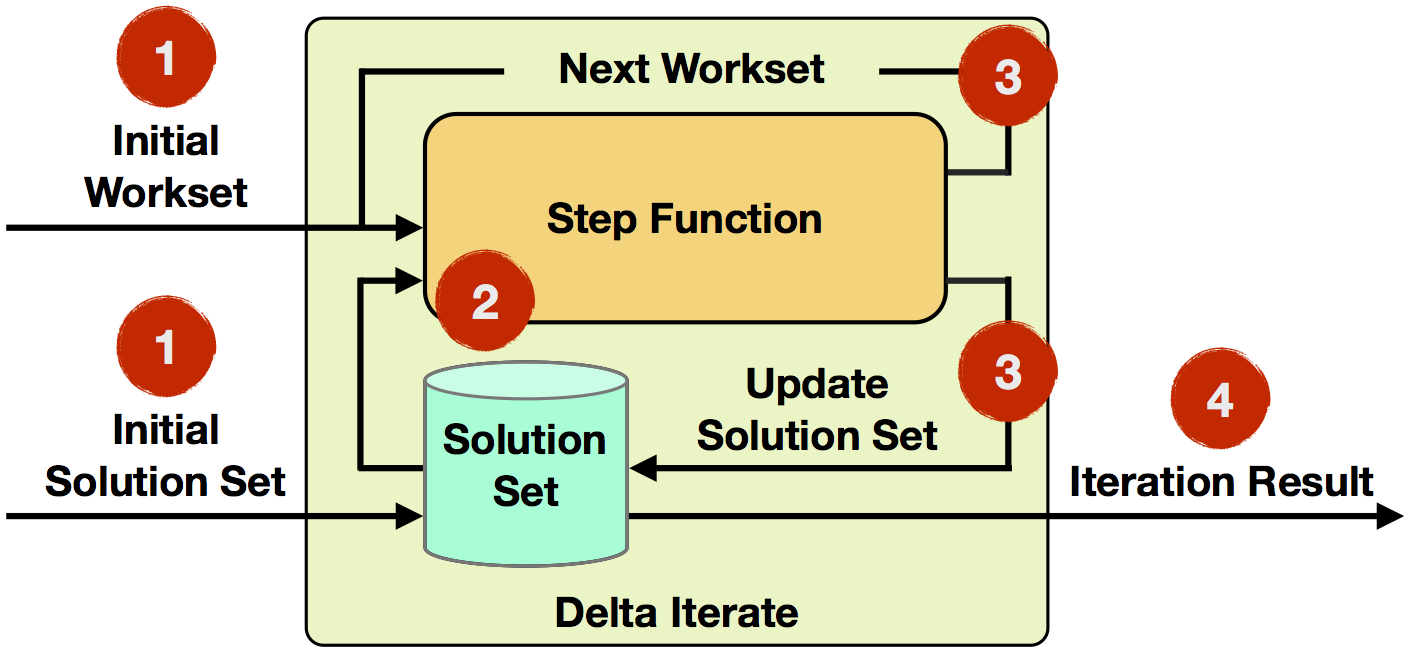
\includegraphics[width=0.48\textwidth]{iterations_delta_iterate_operator}
\end{figure}

\textbf{1. Iteration Input:} The initial workset and solution set are read from data sources or previous operators, as input to the first iteration. 

\textbf{2. Step Function:} The step function will be executed in each iteration.

\textbf{3. Next Workset/Update Solution Set:} The next workset drives the iterative computation and will be fed back into the next iteration. Furthermore, the solution set will be updated and implicitly forwarded.

\textbf{4. Iteration Result:} After the last iteration, the solution set is written to a data sink or used as input to following operators. The default termination condition for delta iterations is specified by the empty workset convergence criterion and a maximum number of iterations. The iteration will terminate when a produced next workset is empty or when the maximum number of iterations is reached. It is also possible to specify a custom aggregator and convergence criterion.

\subsubsection*{Implementation}
After we got our sequence database with ordered itemsets from the InputDecoder we flatMap the database to generate the initial workset for DeltaIteration. The InitialWorkSetExpander creates an entry for the first occurrence of each item in a sequence and stores it as Tuple5 $\left\langle \text{prefix, postfix, 1, joinPrefix, joinParentPrefix}\right\rangle$. Prefix and postfix are stored as Integer arrays, where the prefix is the single item and the postfix is the rest of the sequence after the prefix. JoinPrefix and joinParentPrefix are String representations of the prefix and the parent prefix, and are used to achieve better joining performances.\\
The solution set is initialized as empty dataset of the format Tuple4 $\left\langle \text{prefix, count, joinPrefix, joinParentPrefix}\right\rangle$.

With the initial workset and solution set the frequent pattern mining DeltaIteration is started and proceeded until the empty workset convergence criterion is met. The step function itself is divided into three steps.

\textit{Step 1: Create the solution set.} In this step the workset is grouped by its joinPrefix and the support of each prefix is summed up. Afterwards the infrequent prefixes, which don't meet the threshold, are filtered out. The remaining frequent patterns define the solution set of this iteration.

\textit{Step 2: Create the purify set.} A DataSet $\left\langle \text{joinParentPrefix, baseItemSet}\right\rangle$ which holds the frequent length 1 items of each parent prefix is created. Therefore the solution set is grouped by its joinParentPrefix and the last prefix items are extracted and stored as baseItemSet.

\textit{Step 3: Create the new workset.} To create the workset for the next iteration three steps are executed.\\
First, the infrequent prefixes are filtered out by joining by the solution set's and workset's joinPrefix.\\
Second, the infrequent base items of each postfix are filtered out by joining by the purify set's and workset's joinParentPrefix and by filtering those postfix items which aren't in the baseItemSet.\\
This significantly reduces the amount of further projections, which are performed in the third step. Here each remaining Tuple gets flatMapped similar to the initial workset projection. For each first occurrence of each item in the postfix a new Tuple5 $\left\langle \text{prefix+item, postfix, 1, joinPrefix+item, joinPrefix}\right\rangle$ is created.

After the DeltaIteration has finished the found frequent patterns are collected, ordered by its prefixes and written to a result file.

The source code of this implementation can also be found in our Github repository. \cite{GithubIterative}

\section{Experimental evaluation}
There are two factors of our algorithms we wanted to evaluate, correctness and performance. The correctness criterion was met by manually comparing the results of the three sample databases of the DummyInputDecoder with our result files.\\
To evaluate how performant our algorithm worked we compared it to Apache Spark's reference implementation,  with and without pseudoprojection, \cite{SparkPrefixSpan} and a local implementation of the PrefixSpan algorithm in pure Java. \cite{GithubPureJava}\\
To be comparable we transformed the BigBench datasets of scale factor 1 and 100 into our plain data format, which can be used by all four implementations without further pre-processing. The 88.5MB file of scale factor 1 was transformed to a plain file of 3.9 MB and the 14.7GB file of scale factor 100 was transformed to a plain file of 689MB. The execution times of each implementation can be found in the table below.

\begin{table}[h]
\centering
\begin{tabular}{l|r|r}
 & sf 1 & sf 100 \\\hline
Pure Java & 3.3 sec & 1.1 h \\\hline
Flink Recursive& 2385 sec & --- \\\hline
Flink Iterative& 73 sec & Exception\\\hline
Spark with & \multirow{2}{*}{36 sec} & \multirow{2}{*}{Exception} \\
pseudoprojection & & \\\hline
Spark without & \multirow{2}{*}{81 sec} & \multirow{2}{*}{$>$ 9 h} \\
pseudoprojection & & 
\end{tabular}
\end{table}

As the recursive approach lasted disproportionate long at scale factor 1, we resigned to execute it at scale factor 100. We terminated the Spark execution without pseudoprojection after 9 hours for the same reason. The exceptions thrown at scale factor 100 were both runtime exceptions caused by exceeding the hard drive memory.\\
The Flink and Spark implementations were executed at the ``IBM Cluster" of TU-Berlin. 48 executor cores were assigned to each task, which was executed on 8 processing nodes in parallel. At least 10GB of dedicated RAM was provided by each processing node to execute the implementations. \\
The pure Java implementation was executed on a single Intel Core i5 system with 4GB dedicated RAM and one dedicated core for the execution.


\section{Conclusion}
Both the Flink and Spark implementations aren't yet able to process large amounts of sequences. They both state runtime exceptions due to exceeding the hard drive memory, even if enough physical memory is provided. The most propable reason we found were serialization issues caused by the large worksets created during the flatMap phases. 

As a result we weren't able to compare Spark's and Flink's performance sufficiently and could only deduct from the execution times of sacle factor 1. They state out that pseudoprojection is much more efficient than MapReduce techniques if the datasets fit into main memory. Also the combination of MapReduce for larger sequences and pseudoprojection for those which fit into RAM is more efficient than just using MapReduce techniques.\\
If we compare just the MapReduce capabilities of Spark's implementation and Flink's iterative one, Flink was around 10\% faster than Spark. Our recursive implementation was the least efficient, because Flink needed to read the whole sequence database again from the data source in each recursion call.

\subsubsection*{Missing Flink features}
To implement a more efficient algorithm we missed some key functionalities, which aren't yet provided by Flink.

To improve the performance of our recursive approach, a feature to explicitly write the whole sequence database into RAM, like Spark's ``.persist(StorageLevel.MEMORY\_AND\_DISK)", would be helpful.

To follow a better divide and conquer approach during the flatMap phase, a feature to iterate over each single item in a dataset and perform MapReduce functions on this single item would be better for our algorithm. Spark has an ``.forearch()" function for this purpose and uses it in its PrefixSpan implementation.

Spark also offers the opportunity to define unique item ids for better joining performance. We first used the prefix integer array as join key, but it turned out to be inefficient. Therefore we needed to introduce a String representation of the prefix to achieve a better joining performance with the drawback of redundant data.

The last problem we faced was to append information to a dataset outside of our delta iteration and to use it as a data sink afterwards. It's currently not supported by Flink. Therefore we couldn't finish our implementation with local pseudoprojection \cite{GithubIterativePseudo} in an efficient way.\footnote{The former commit has a work-around, which is executable but slower.}

\begin{thebibliography}{99}
\raggedright
\bibitem{PrefixSpan} J. Pei, J. Han, B. Mortazavi-Asl, J. Wang, H. Pinto, Q. Chen, U. Dayal, M. Hsu, Mining Sequential Patterns by Pattern-Growth: The PrefixSpan Approach
\bibitem{Flink} Apache Flink - Homepage, \url{https://flink.apache.org/}, last accessed 10.02.2016
\bibitem{Spark} Apache Spark - Homepage, \url{https://spark.apache.org/}, last accessed 10.02.2016
\bibitem{BigBench} Big Data Benchmark for BigBench, \url{https://github.com/intel-hadoop/Big-Data-Benchmark-for-Big-Bench}, last accessed 07.02.2016
\bibitem{IBMDataGenerator} Download site of IBM's quest data generator, \url{http://forum.ai-directory.com/read.php?5,33}, last accessed 07.02.2016
\bibitem{GithubRecursive} GitHub Repository - Recursive Implementation, \url{https://github.com/sneJ-/IMPRO-3.WS15/blob/assignment-3/prefixSpan/src/main/java/prefixSpan/PrefixSpan.java}, last accessed 10.02.2016
\bibitem{GithubIterative} GitHub Repository - Iterative Implementation, \url{https://github.com/sneJ-/IMPRO-3.WS15/blob/assignment-3/prefixSpan/src/main/java/prefixSpan/PrefixSpanDelta7.java}, last accessed 10.02.2016
\bibitem{SparkPrefixSpan} Reference implementation of PrefixSpan in Apache Spark, \url{https://spark.apache.org/docs/1.6.0/mllib-frequent-pattern-mining.html#prefixspan}, last accessed 08.02.2016
\bibitem{GithubPureJava} GitHub Repository - Pure Java Implementation, \url{https://github.com/sneJ-/IMPRO-3.WS15/blob/assignment-3/prefixSpan/src/main/java/prefixSpanPrototype/PrefixSpanPrototypePlain.java}, last accessed 08.02.2016
\bibitem{GithubIterativePseudo} GitHub Repository - Iterative Pseudoprojection Implementation, \url{https://github.com/sneJ-/IMPRO-3.WS15/blob/assignment-3/prefixSpan/src/main/java/prefixSpan/PrefixSpanDeltaLocal.java}, last accessed 14.02.2016
\end{thebibliography}
\end{document}